\documentclass[posterIC]{a0poster}
\usepackage{alltt}
\usepackage{color}
\usepackage{times}
\usepackage{a0poster}
\usepackage{graphicx,amsmath,amsfonts,amssymb,amscd,bezier,amstext,makeidx}
\usepackage[brazil]{babel}
\usepackage[utf8]{inputenc}
\usepackage{psfrag}
\usepackage{posterbox}
\usepackage{multicol}
\usepackage{url}

\renewcommand{\baselinestretch}{1.2}     

\setlength{\topmargin}{1.0cm}
\def\bordercolor{white}

\begin{document}
\vspace{5cm}
\title{\veryHuge{\textit{Workflow} autonômico para aplicações de \textit{Machine Learning} utilizando métricas de \textit{Fairness}}}

\author{\Large Autor: Thales Eduardo Nazatto (tenazatto@gmail.com) \paragraph

\vspace{-1.3cm} Orientador(es): Cecília Mary Fischer Rubira (cmrubira@ic.unicamp.br), Leonardo Montecchi (leonardo.montecchi@ntnu.no) \paragraph

Palavras-chave: \textit{Workflow}, \textit{Machine Learning}, Inteligência Artificial, Computação Autônoma, Métricas de \textit{Fairness}
}
\makeheader

\begin{multicols}{2}
\section{Introdução}

O uso de Inteligência Artificial (IA) envolvendo grandes volumes de dados vem crescendo conforme nossa sociedade migra processos manuais de trabalho para soluções digitais e necessita de tomadas de decisão mais rápidas e assertivas, mas, devido a barreiras éticas e legais, métricas usadas inicialmente para definir a eficácia de um algoritmo se mostraram limitadas para medir vieses que refletem a sociedade de maneira que não era esperada pelos desenvolvedores da solução. Para resolver tal problema, novos algoritmos foram desenvolvidos e um novo conjunto de métricas, denominado como métricas de Fairness, é utilizado para determinar um equilíbrio entre grupos que sofrem discriminações. Entretanto, novos problemas surgem com a introdução deste novo conjunto de algoritmos e métricas, como a piora nas métricas tradicionais de avaliação e aumento de combinações de algoritmos utilizados no processo, aumentando a complexidade da análise do Cientista de Dados para obter modelos de forma otimizada.

\section{Objetivo}

O objetivo deste trabalho é desenvolver uma estrutura de \textit{Workflow} para aplicações de \textit{Machine Learning} que seja completamente autônoma, por três fatores principais:

\begin{itemize}
\item Facilitar a criação de modelos justos e confiáveis com a automatização da escolha dos algoritmos, cuja complexidade aumenta com a escolha dos algoritmos a serem utilizados e suas execuções nas etapas corretas do processo, onde eles foram escolhidos para atuar.
\item Estabelecer um balanceamento entre métricas para avaliar bons modelos com métricas para avaliar modelos justos.
\item Considerar proveniência de dados como requisito no design de uma solução de IA, e como uma alternativa a \textit{Explainable AI} através da utilização de metadados.
\end{itemize}

\section{Metodologia}

Foi desenvolvido um sistema, que pode ser dividido em 4 etapas principais: 

\begin{itemize}
    \item {\textbf{Engenharia de dados:}} Etapa criada com o objetivo de simular processos de transformação e limpeza de dados.
    \item {\textbf{\textit{Workflow} de IA:}} Etapa para execução de um \textit{Workflow} que simula o desenvolvimento de uma aplicação automatizada de IA, desde uma categorização dos dados mais específica do que na etapa anterior, passando pelo algoritmo utilizado e finalizando obtendo métricas para determinar qualidade do resultado final.
    \item {\textbf{Autonomia do \textit{Workflow}:}} Etapa que automatiza todas as etapas do \textit{Workflow} através de um componente, com o objetivo de evitar com que perca-se tempo em execuções manuais que podem demorar dependendo do algoritimo e do conjunto de dados utilizado.
    \item {\textbf{Interface Humano-Computador:}} Etapa criada com o objetivo de simular a etapa anterior, porém de modo a proporcionar uma experiência de usuário mais simples e intuitiva, onde sua integração com as outras etapas é mostrada na Figura \ref{fig:SystemCommunication}. É dividida em duas partes:
    \begin{itemize}
        \item {\textbf{Frontend:}} Parte visual, exibida em um navegador.
        \item {\textbf{Backend:}} Parte onde o Frontend se comunica para obter os dados para auxiliar a montagem do visual e executa o componente utilizado na etapa de autonomia, de forma que corresponda a configurações utilizadas por ela.
    \end{itemize}
\end{itemize}

\begin{figure}
\centering
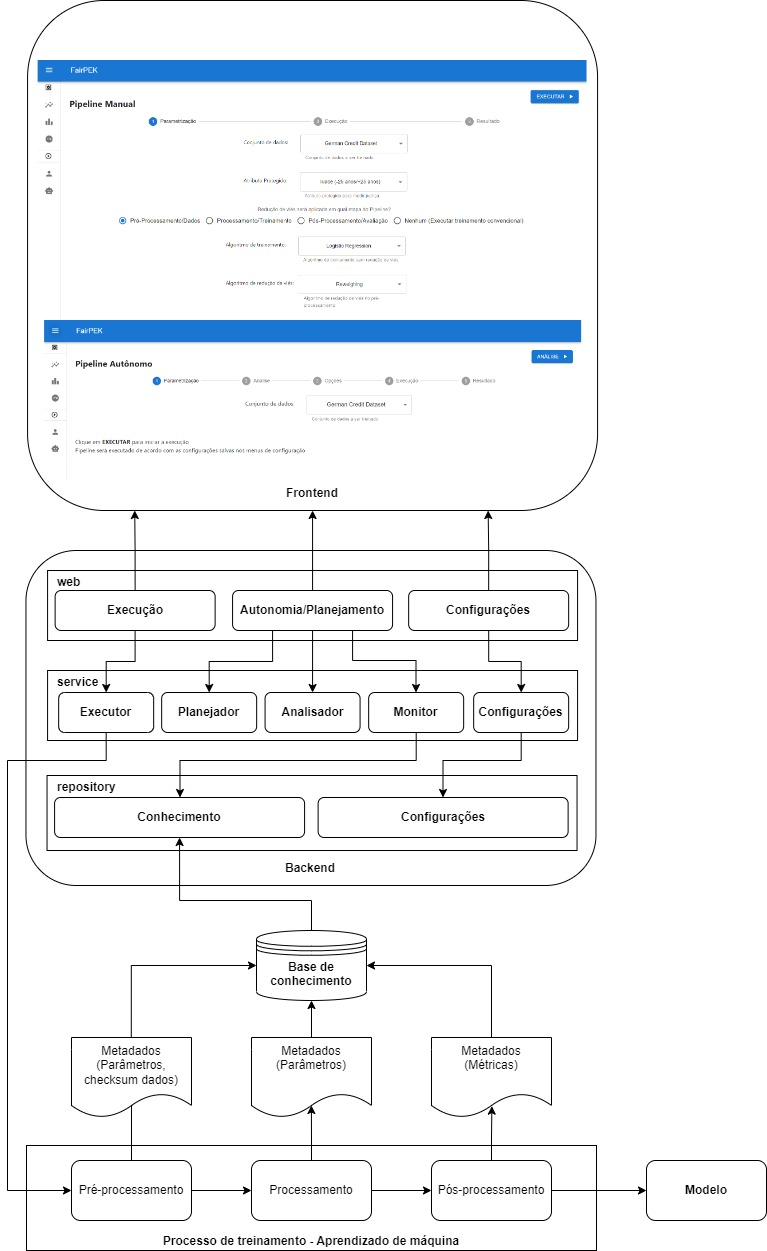
\includegraphics[scale=0.4]{images/backend-frontend-ml.jpg}
\caption {Comunicação entre interface, autonomia e \textit{Workflow} de IA}
\label{fig:SystemCommunication}
\end{figure}

Para o desenvolvimento do \textit{workflow}, será utilizada a arquitetura \textit{Pipe-and-Filter}. Para a autonomia deste, será criado um componente utilizando a arquitetura MAPE-K~\cite{IBM_2005} para analisar uma base de conhecimento e prover o melhor pipeline seguindo regras pré-determinadas. Para a interface, ela foi criada nos moldes de uma aplicação web. O código deste desenvolvimento foi disponibilizado no GitHub (\url{https://github.com/tenazatto/MsC}) para avaliação e testes em estudos posteriores. 

\section{Resultados}

Foram realizados estudos de caso para verificar a viabilidade da arquitetura MAPE-K na autonomia e a capacidade de evolução para o uso de novos algoritmos e conjuntos de dados. Foi atribuída uma pontuação de 0 a 1000 no cálculo realizado pela análise.

\begin{center}
\label{tbl:ScoreMAPEKGeral5050}
  \resizebox{\linewidth}{!}{%
\begin{tabular}{c|c|c|c|c|c|c}
\multicolumn{4}{c|}{Workflow} & \multicolumn{3}{c}{Pontuação} \\
\hline
Atributo protegido & Pré-processamento & Treinamento & Pós-processamento & Performance & Fairness & \textbf{Geral} \\
\hline
Idade & Nenhum & Regressão Logística & Equalized Odds & 968 & 860 & \textbf{914} \\
Nacionalidade & Nenhum & Random Forest & Calibrated Equalized Odds & 902 & 922 & \textbf{912} \\
Nacionalidade & Nenhum & Gradient Boosting & Calibrated Equalized Odds & 870 & 925 & \textbf{898} \\
Idade & Nenhum & Gradient Boosting & Equalized Odds & 927 & 862 & \textbf{894} \\
Idade & Reweighing & Gradient Boosting & Nenhum & 804 & 931 & \textbf{868} \\
\end{tabular}}
\end{center}

É possível ver que há uma diversidade entre os parâmetros do workflow e suas pontuações entre métricas de performance e métricas de \textit{Fairness}, a arquitetura MAPE-K se mostra viável para efetuar um balanceamento. Com diferentes definições de pesos para as métricas, é possível calibrar qual a melhor escolha dependendo do contexto do problema.

Como exemplo para evolução, foram necessárias modificações para adicionar um novo conjunto de dados como opção no \textit{Workflow}. Estas foram contadas de acordo com seus \textit{commits} realizados no repositório e exibidos na tabela abaixo:

\begin{center}
\label{tbl:ManutencaoPipelineDataset}
  \resizebox{\linewidth}{!}{%
\begin{tabular}{c|c|c|c|c|c|c}
Parte do Sistema & Linhas alteradas & Total de linhas & Arquivos alterados & Total de arquivos & \% linhas alteradas & \% arquivos alterados \\
\hline
Engenharia de Dados & 122 & 277 & 2 & 3 & \textbf{44,04\%} & \textbf{66,67\%} \\
\textit{Workflow} de IA & 76 & 1982 & 5 & 38 & \textbf{3,84\%} & \textbf{13,16\%} \\
Autonomia do \textit{Workflow} & 0 & 457 & 0 & 10 & \textbf{0,00\%} & \textbf{0,00\%} \\
Interface Humano-Computador (\textit{Frontend}) & 13 & 2905 & 2 & 14 & \textbf{0,45\%} & \textbf{14,29\%} \\
Interface Humano-Computador (\textit{Backend}) & 4 & 432 & 1 & 7 & \textbf{0,93\%} & \textbf{14,29\%} \\
\hline
\textbf{TOTAL} & \textbf{215} & \textbf{6053} & \textbf{10} & \textbf{72} & \textbf{3,55\%} & \textbf{13,89\%} \\
\end{tabular}}
\end{center}

Destas modificações, percebe-se que a grande maioria delas está relacionada a parte de engenharia de dados. Mesmo no \textit{Workflow} de IA, a maior parte dessas linhas não está relacionada a sua estrutura e sim a uma etapa de adaptação dos dados ao atributo protegido, necessário para algoritmos dedicados a reduzir viés nos dados. A etapa de autonomia e a Interface Humano-Computador exigiram poucas ou nenhuma alteração e em poucos arquivos, comprovando que a modularização das arquiteturas escolhidas facilita a manutenção do sistema e que a autonomia não é afetada por evoluções no \textit{Workflow}.

\section{Conclusões}

Esta pesquisa mostra que a escolha da arquitetura \textit{Pipe-and-Filter} se mostra favorável para o desenvolvimento de um \textit{workflow} para aplicações envolvendo IA, permitindo que ele seja modular e que sejam feitas evoluções sem exigir grandes esforços. O uso da arquitetura MAPE-K também se mostrou favorável, permitindo diversos resultados para diferentes contextos de problema e uma simplificação da análise realizada pelo Cientista de Dados, podendo resultar em economia de tempo. Ela também possibilitou um balanço entre performance e justiça através da adição de pesos para cada métrica na parte de análise. Embora os pesos não sejam parte da arquitetura, a divisão presente na arquitetura permite que o desenvolvimento seja pensado de maneira mais clara.

Embora a proveniência de dados não teve o mesmo efeito da aplicação de um método feito para \textit{Explainable AI}, a obtenção de metadados do \textit{workflow} se mostrou essencial para alimentar o componente baseado na arquitetura MAPE-K e possibilitou a análise e tomadas de decisão baseadas em dados. É possível realizar análises mais detalhadas conforme novas execuções forem realizadas, consequentemente podendo resultar em melhores escolhas de algoritmos para contextos distintos, e até considerar novas aplicações de IA caso o volume de dados seja consideravelmente grande. Posteriormente, é possível também rever quais dados podem ser adicionados para que o objetivo de \textit{Explainable AI} possa ser alcançado de maneira satisfatória.

\bibliographystyle{plainnat}
\bibliography{poster}
\end{multicols}

%\begin{center}
%	\vspace{30cm}
%	{\Huge 
%		\underline{\textbf{Diretrizes:}}\\
%		\begin{itemize}
%			\item Contemplar os seguintes itens: contexto (com a motivação e a definição do problema), objetivos, método, resultados e conclusões.
%			\item Tópicos devem ser abordados de maneira objetiva.
%			\item Letras legíveis e com uso de figuras explicativas no lugar de texto, sempre que possível.
%			\item Usar uma ou duas colunas.	
%		\end{itemize}
%	}
%\end{center}


%\col{{
%\vspace{1.0cm}
%\begin{center}
%\Large{\textbf{\textcolor[rgb]{1.00,1.00,1.00}{Secao 1}}}
%\end{center}
%}}

%\col{ \vspace{1.0cm} {

%\begin{center}
%\Large{\textbf{\textcolor{red}{Secao 2}}}
%\end{center}

%\col{ { \vspace{1.0cm}
%\begin{center}
%\Large{\textbf{\textcolor[rgb]{1.00,1.00,1.00}{Secao 3}}}
%\end{center}
\makefooter

\end{document}

